\documentclass[12pt]{article}
\usepackage{amsmath}
\usepackage{graphicx}
%opening
\title{Ley de Ohm - Potencia en resistencias}
\author{Juan Barbosa - 201325901}

\begin{document}

\maketitle

\section{Resistencia equivalente}
Para el primer circuito es necesario tener en cuenta que las resistencias \verb|R1| y \verb|R2| comparten uno de sus nodos sin que exista un tercer elemento en el mismo, por lo cual se encuentran en serie.
\begin{equation}
	R_{eq}=R_1+R_2=10\text{k}+4.7\text{k}=14.7\text{k}\Omega
\end{equation}

En el segundo circuito las resitencias \verb|R1| y \verb|R2| comparten ambos nodos, por lo cual se encuentran en paralelo.
\begin{equation*}
	\dfrac{1}{R_{eq}}=\dfrac{1}{R_{1}}+\dfrac{1}{R_{2}}=\dfrac{R_1+R_2}{R_1R_2}
\end{equation*}
\begin{equation}\label{eq: paralelo}
	R_{eq}=\dfrac{R_1R_2}{R_1+R_2}=\dfrac{1\text{k}\times150}{1\text{k}+150}\approx 130.4 \Omega
\end{equation}

El \'ultimo circuito requiere realizar pasos intermedios.
\begin{center}
	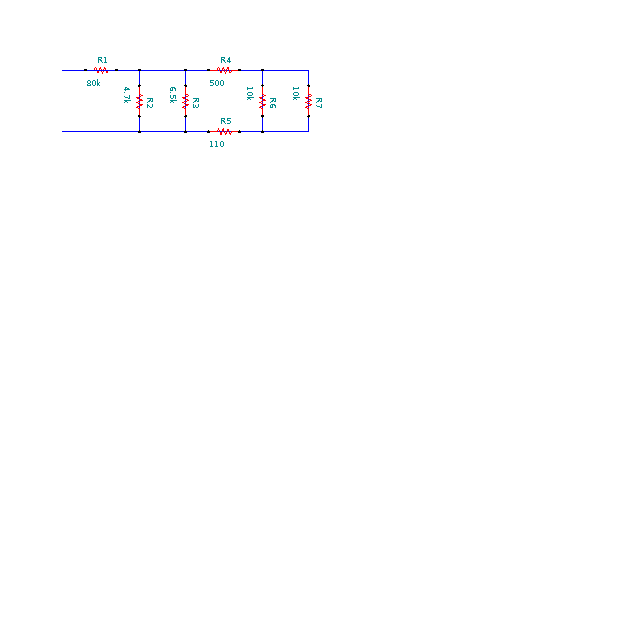
\includegraphics[scale=2]{Circuito1.pdf}
\end{center}

En primer lugar se obtienen dos resistencias equivalentes de la pareja de resistencias (\verb|R2|, \verb|R3|), y (\verb|R6|, \verb|R7|), las cuales se encuentran en paralelo.
\begin{center}
	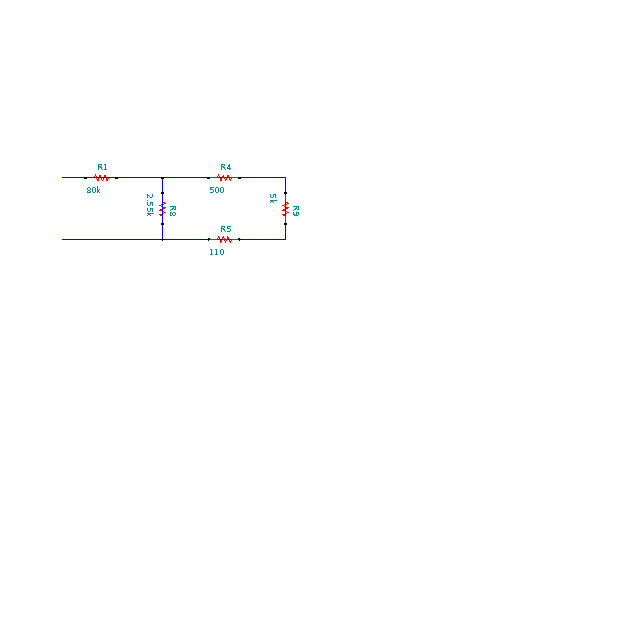
\includegraphics[scale=2]{Circuito2.pdf}
\end{center}

Donde usando la ecuaci\'on (\ref{eq: paralelo}) se obtiene una resistencia equivalente \verb|R8| y \verb|R9| con valores de 2.55 k$\Omega$ y 5 k$\Omega$. En este punto se tienen tres resistencias en serie (\verb|R4|, \verb|R9|, y \verb|R5|).
\begin{center}
	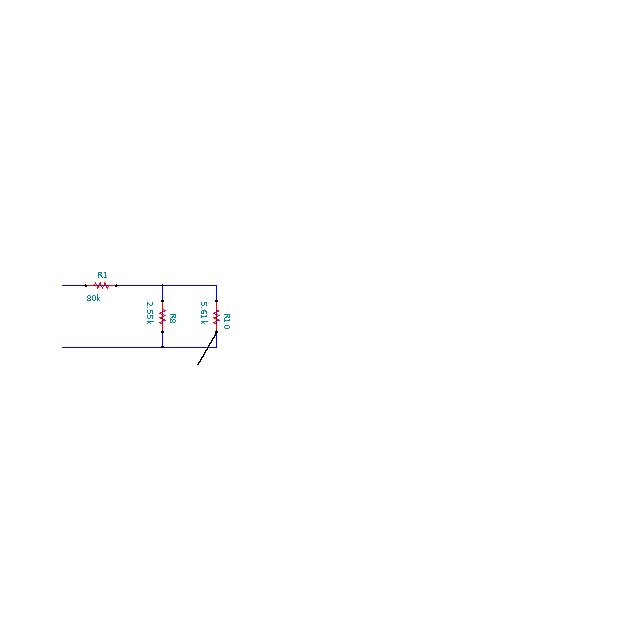
\includegraphics[scale=2]{Circuito3.pdf}
\end{center}

Sumando los valores de las resistencias se obtiene el valor equivalente \verb|R10| con 5.61 k$\Omega$. El circuito se encuentra bastante simplificado en este punto, y es f\'acil ver que las resistencias \verb|R8| y \verb|R10| se encuentran en paralelo.
\begin{center}
	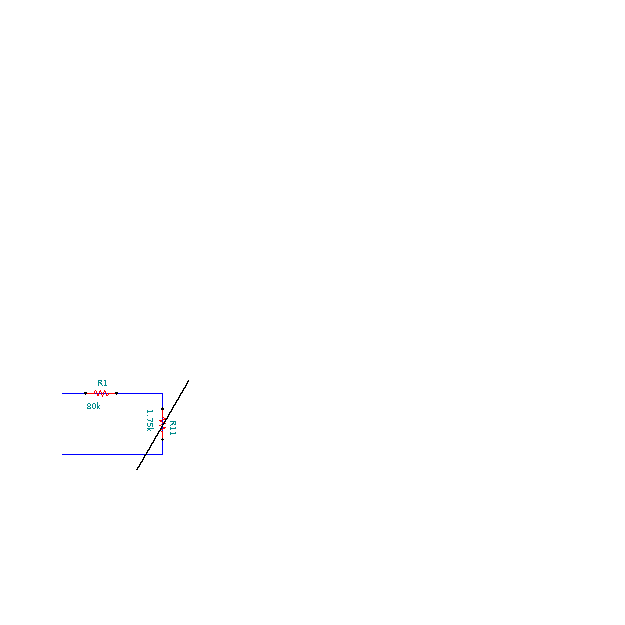
\includegraphics[scale=2]{Circuito4.pdf}
\end{center}

La resistencia equivalente tiene un valor de 1.75 k$\Omega$. Finalmente las resistencias \verb|R1| y \verb|R11| se encuentran en serie, de donde resulta f\'acil calcular la resistencia equivalente de la totalidad del circuito, con un valor de 81.75 k$\Omega$.
\begin{center}
	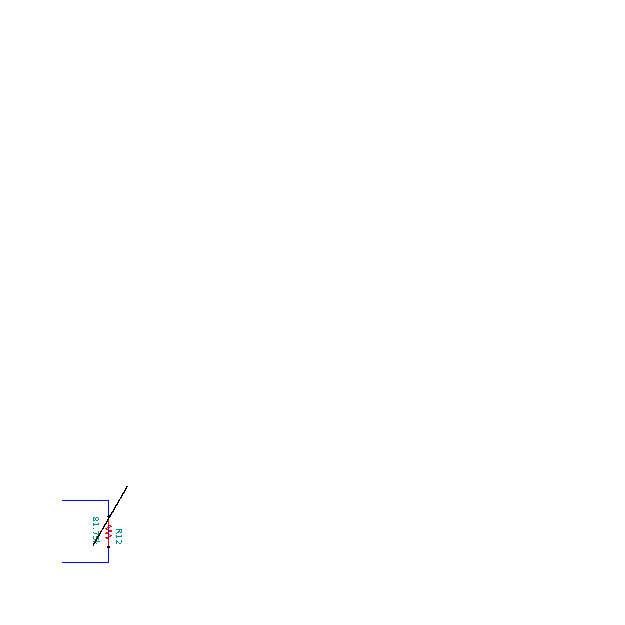
\includegraphics[scale=1.5]{Circuito5.pdf}
\end{center}
\end{document}
